\newif\ifalone
\alonefalse
\ifalone
\documentclass{article}
\usepackage{graphicx}
\usepackage{natbib}
\usepackage{amsfonts}
\usepackage{amssymb}
\usepackage{amsthm}
\usepackage{bm}
\usepackage{Sweave}
\usepackage{lscape}
\usepackage{makeidx}
\usepackage{hyperref}

\let\proglang=\textsf
\newcommand{\pkg}[1]{{\fontseries{b}\selectfont #1}}
  \hypersetup{%
    hyperindex = {true},
    colorlinks = {true},
    linktocpage = {true},
    plainpages = {false},
    linkcolor = {blue},
    citecolor = {blue},
    urlcolor = {red},
    pdfstartview = {Fit},
    pdfpagemode = {UseOutlines},
    pdfview = {XYZ null null null}
  }

\title{Parameter Expansion}
\author{Jarrod Hadfield (\texttt{j.hadfield@ed.ac.uk})}

\begin{document}
\maketitle
\else
\chapter{Parameter Expansion}
\label{secPX}
\fi

As the covariance matrix approaches a singularity, the mixing of the chain can become notoriously slow. This problem is often encountered in single-response models when a variance component is small and the chain becomes stuck at values close to zero.  Similar problems occur for the EM algorithm and \citet{Liu.1998} introduced parameter expansion to speed up the rate of convergence. The idea was quickly applied to Gibbs sampling problems \citep{Liu.1999} and has now been extensively used to develop more efficient mixed-model samplers \citep[e.g.][]{vanDyk.2001, Gelman.2008b, Browne.2009}.\\

The columns of the design matrix (${\bf W}$) can be multiplied by the non-identified working parameters ${\bm \alpha} = \left[1,\ \alpha_{1},\ \alpha_{2},\ \dots \alpha_{k}\right]^{'}$:

\begin{equation} 
{\bf W}_{\alpha} = \left[{\bf X}\ {\bf Z}_{1}\alpha_{1}\ {\bf Z}_{2}\alpha_{2}\ \dots\ {\bf Z}_{k}\alpha_{k}\right]
\label{wstar}
\end{equation}

where the indices denote submatrices of ${\bf Z}$ which pertain to effects associated with the same variance component. Replacing  ${\bf W}$ with ${\bf W}_{\alpha}$ in Section \ref{MCMC-app}, we can sample the new location effects  ${\bm \theta}_{\alpha}$, and rescale them to obtain ${\bm \theta}$:

\begin{equation} 
{\bm \theta} = ({\bf I}_{n_{\bf \beta}}\oplus_{i=1}^{k}{\bf I}_{n_{{\bf u}_{i}}}\ \alpha_{i}){\bm \theta}_{\alpha}
\end{equation}

where the identity matrices are equal in dimension to $n_{x}$ the number of elements in the subscripted parameter vector $x$.\\ 

Likewise, the (co)variance matrices can be rescaled by the set of $\alpha$'s associated with the variances of a particular variance structure component (${\bm \alpha}_{\mathcal{V}}$):

\begin{equation} 
{\bf V} = Diag({\bm \alpha}_{\mathcal{V}}){\bf V}_{\alpha}Diag({\bm \alpha}_{\mathcal{V}})
\end{equation} 

The working parameters are not identifiable in the likelihood, but do have a proper conditional distribution.  Defining ${\bf X}_{\alpha}$ as an $n\times( k+1)$ design matrix,  with each column equal to the sub-matrices in Equation \ref{wstar} post-multiplied by the relevant sub-vectors of ${\bm \theta}_{\alpha}$, we can see that ${\bm \alpha}$ is a vector of regression coefficients: 

\begin{equation}
\begin{array}{rl}
\bf{l} =& {\bf X}_{\alpha}{\bm \alpha}+\bf{e}\\
\end{array}
\end{equation}

and so the methods described in Section \ref{MCMC-app} can be used to update them.\\ 

\texttt{MCMCglmm} uses a (multivariate) normal prior for the $\alpha$'s and these are set by passing additional arguments to each element of the prior {\bf G}-structure. As with the priors for the fixed effects, we need to specify the prior mean (\texttt{alpha.mu}) and the prior covariance matrix (\texttt{alpha.V}). In Section \ref{secPX-p} I discuss what this prior means in the context of posterior inference, but for now we will look into the ability of parameter expansion to improve mixing.

\section{Variances close to zero}

  To illustrate the ability of parameter expansion to improve mixing, we will fit  two models that estimate the between mother variation in offspring sex ratio in Blue tits.    To fit a parameter expanded model we need to specify a non-null prior covariance matrix for the $\alpha$'s.  To begin, we will specify a diffuse prior by setting the variance to be large:  

\begin{Schunk}
\begin{Sinput}
> BTdata$sex[which(BTdata$sex == "UNK")] <- NA
> BTdata$sex <- gdata::drop.levels(BTdata$sex)
> prior1b = list(R = list(V = 1, fix = 1), G = list(G1 = list(V = 1, 
+     nu = 1, alpha.mu = 0, alpha.V = 1000)))
> m7b.1 <- MCMCglmm(sex ~ 1, random = ~dam, data = BTdata, family = "categorical", 
+     prior = prior1b, verbose = FALSE)
\end{Sinput}
\end{Schunk}

We can also fit a standard model without parameter expansion, and our choice of prior should become clear from reading Section \ref{secPX-p}:

\begin{Schunk}
\begin{Sinput}
> prior2b = list(R = list(V = 1, fix = 1), G = list(G1 = list(V = 1e-10, 
+     nu = -1)))
> m7b.2 <- MCMCglmm(sex ~ 1, random = ~dam, data = BTdata, family = "categorical", 
+     prior = prior2b, verbose = FALSE)
\end{Sinput}
\end{Schunk}

The prior densities in the two models are very similar across the range of variances that have reasonable posterior support, and running the models for long enough will verify that they are sampling from very similar posterior densities. However, the mixing properties of the two chains are very different, with the non-parameter expanded chain (in red) getting stuck at values close to zero (Figure \ref{sexratio-fig}).\\


\begin{figure}[!h]
\begin{center}
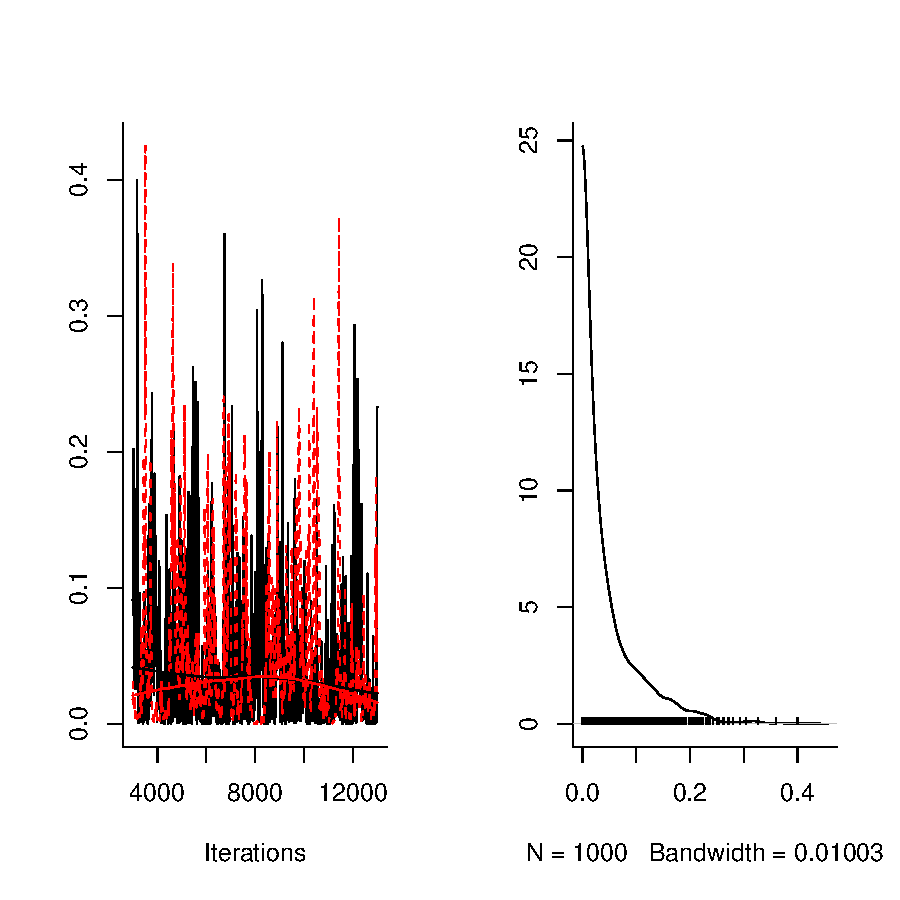
\includegraphics{Lecture8-004}
\end{center}
\caption{Traces of the sampled posterior distribution for between female variance in sex ratio. The black trace is from a parameter expanded model, and the red trace from a non-parameter expanded model.}
\label{sexratio-fig}
\end{figure}

The parameter expanded model is 25\% slower per iteration but the effective sample size is 1.418 times greater:

\begin{Schunk}
\begin{Sinput}
> effectiveSize(m7b.1$VCV[, 1])
\end{Sinput}
\begin{Soutput}
    var1 
116.9204 
\end{Soutput}
\begin{Sinput}
> effectiveSize(m7b.2$VCV[, 1])
\end{Sinput}
\begin{Soutput}
    var1 
82.46342 
\end{Soutput}
\end{Schunk}

\section{Parameter expanded priors}
\label{secPX-p}

The original aim of applying parameter expanded methods to Gibbs sampling was to speed up the convergence and mixing properties of the chain. They achieve this by introducing parameters that are not identified in the likelihood, and for which all information comes from the prior distribution. By placing priors on these parameters we can induce different prior distributions for the variance components. These priors are all from the non-central scaled F-distribution, which implies the prior for the standard deviation is a non-central folded scaled t-distribution \citep{Gelman.2006}.  Without loss of generality we can set \texttt{V=1} in the prior, so that the prior for the variance (\texttt{v}) has density function:

\begin{Schunk}
\begin{Sinput}
> df(v/alpha.V, df1 = 1, df2 = nu, ncp = (alpha.mu^2)/alpha.V)
\end{Sinput}
\end{Schunk}

and the prior for the standard deviation:

\begin{Schunk}
\begin{Sinput}
> 2 * dt(sqrt(v)/sqrt(alpha.V), df = nu, ncp = alpha.mu/sqrt(alpha.V))
\end{Sinput}
\end{Schunk}

where \texttt{v}$>0$.\\

To illustrate I'll use the original Schools example from \citet{Gelman.2006}, the data of which are available through the \proglang{R} library \pkg{R2WinBUGS}:

\begin{Schunk}
\begin{Sinput}
> data(schools)
> head(schools)
\end{Sinput}
\begin{Soutput}
  school estimate   sd
1      A    28.39 14.9
2      B     7.94 10.2
3      C    -2.75 16.3
4      D     6.82 11.0
5      E    -0.64  9.4
6      F     0.63 11.4
\end{Soutput}
\end{Schunk}

In this example the actual data for each school are not presented and we only have two summary statistics: the response variable \texttt{estimate} is the estimated relative effect of Scholastic Aptitude Test coaching programs in 8 \texttt{schools}, and \texttt{sd} is the standard deviation of the test scores within each school. In the original example Gelman focused on the standard deviation of the between school effects, and by fixing the residual variance for each school at its standard deviation squared, we can estimate the between school variance.  

\begin{Schunk}
\begin{Sinput}
> prior1 <- list(R = list(V = diag(schools$sd^2), fix = 1), G = list(G1 = list(V = 1e-10, 
+     nu = -1)))
> m7a.1 <- MCMCglmm(estimate ~ 1, random = ~school, rcov = ~idh(school):units, 
+     data = schools, prior = prior1, verbose = FALSE)
\end{Sinput}
\end{Schunk}

The posterior distribution of the between school standard deviation is shown in Figure \ref{school1-fig} with the flat prior shown as a solid line.\\ 


\begin{figure}[!h]
\begin{center}
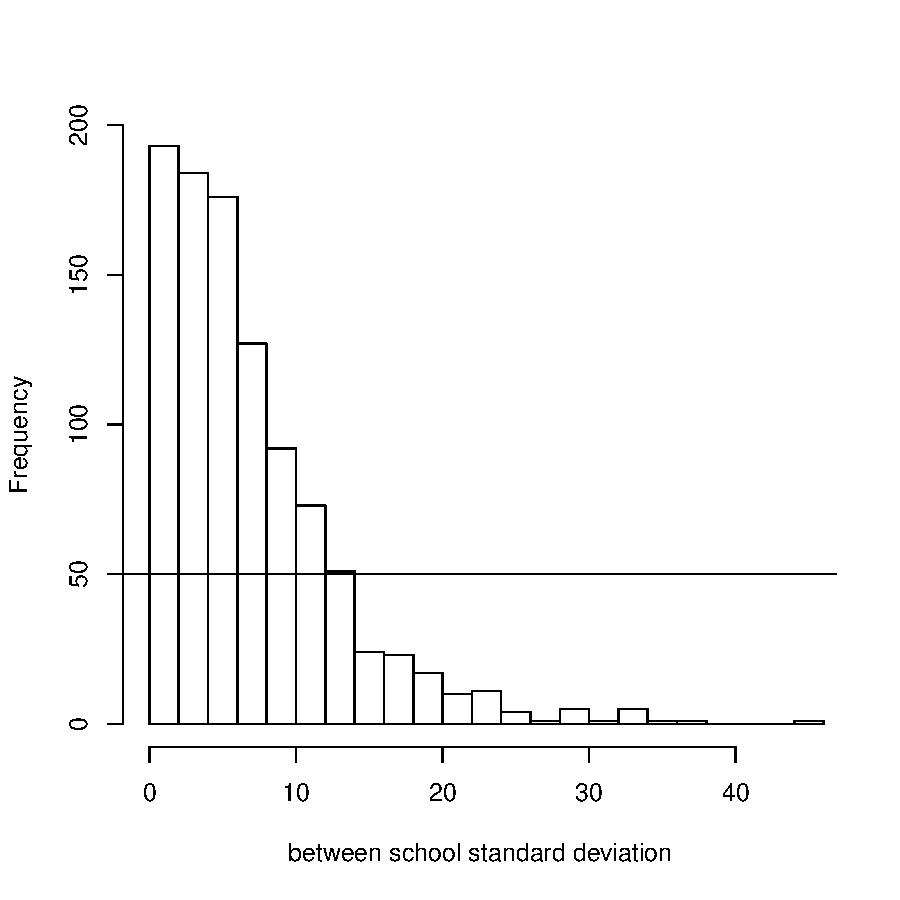
\includegraphics{Lecture8-011}
\end{center}
\caption{Between school standard deviation in educational test scores, with an improper uniform prior}
\label{school1-fig}
\end{figure}

We can also use the inverse-gamma prior with scale and shape equal to 0.001:

\begin{Schunk}
\begin{Sinput}
> prior2 <- list(R = list(V = diag(schools$sd^2), fix = 1), G = list(G1 = list(V = 1, 
+     nu = 0.002)))
> m7a.2 <- MCMCglmm(estimate ~ 1, random = ~school, rcov = ~idh(school):units, 
+     data = schools, prior = prior2, verbose = FALSE)
\end{Sinput}
\end{Schunk}

but Figure \ref{school2-fig} indicates that such a prior in this context may put too much density and values close to zero.\\


\begin{figure}[!h]
\begin{center}
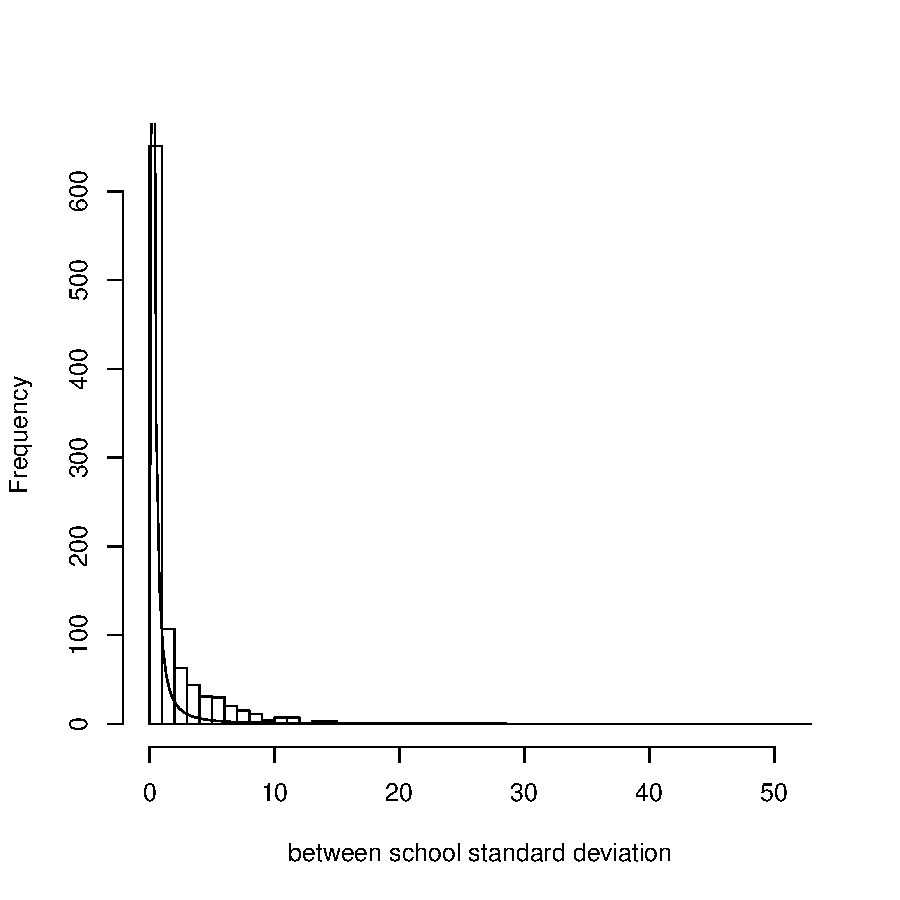
\includegraphics{Lecture8-014}
\end{center}
\caption{Between school standard deviation in educational test scores, with an inverse-gamma prior with shape and scale set to 0.001}
\label{school2-fig}
\end{figure}

For the final prior we have \texttt{V=1}, \texttt{nu=1} and \texttt{alpha.mu=0}.  In this instance the scaled non-central folded $t$ prior for the standard deviation is equivalent to a half-Cauchy distribution with scale equal to $\sqrt{\texttt{alpha.V}}$. Following \citet{Gelman.2006} we use a scale of 25: 

\begin{Schunk}
\begin{Sinput}
> prior3 <- list(R = list(V = diag(schools$sd^2), fix = 1), G = list(G1 = list(V = 1, 
+     nu = 1, alpha.mu = 0, alpha.V = 25^2)))
> m7a.3 <- MCMCglmm(estimate ~ 1, random = ~school, rcov = ~idh(school):units, 
+     data = schools, prior = prior3, verbose = FALSE)
\end{Sinput}
\end{Schunk}

and Figure \ref{school3-fig} shows that the prior may have better properties than the inverse-gamma.


\begin{figure}[!h]
\begin{center}
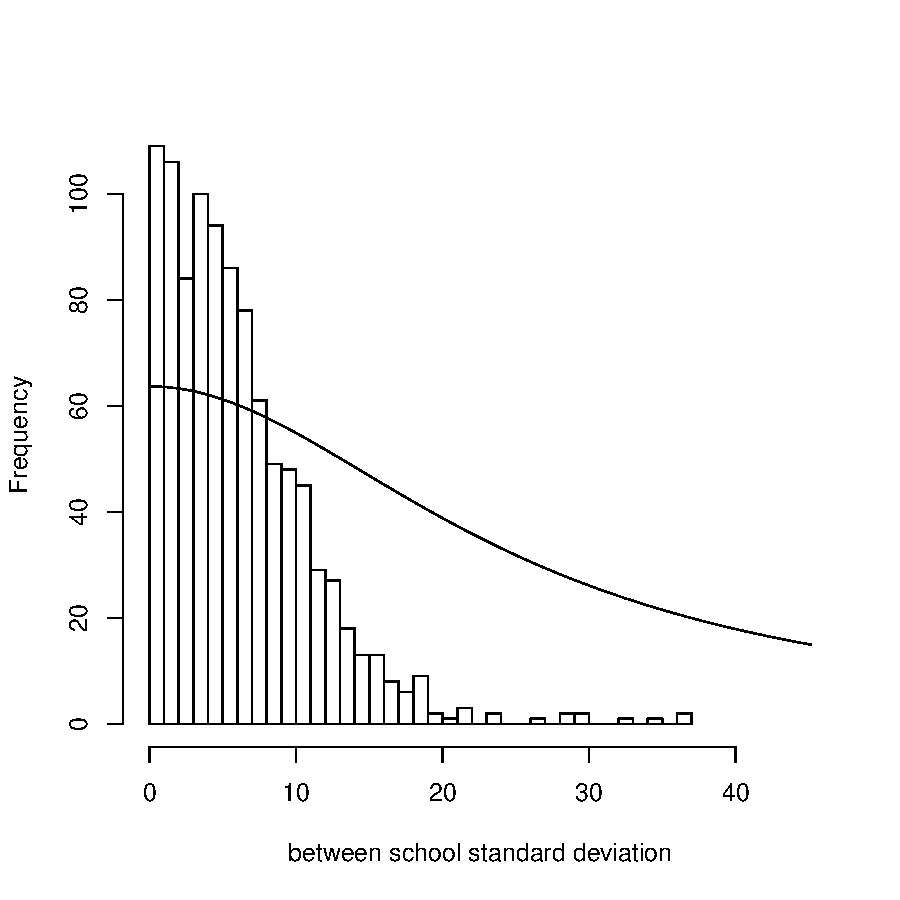
\includegraphics{Lecture8-017}
\end{center}
\caption{Between school standard deviation in educational test scores, with a half-Cauchy prior with a scale of 25.}
\label{school3-fig}
\end{figure}

\subsection{Binary response models}

When analysing binary responses, the residual variance is not identified in the likelihood and without a prior the posterior is improper.  If a weak prior is placed on the residual variance then the chain appears to mix poorly and the MCMC output often looks terrible. However, this poor mixing is in some ways superficial. As discussed in Section \ref{cat-sec} we can rescale the location effects and variances by the estimated residual variance to obtain the posterior distribution for some fixed value of the actual residual variance. For example, we can refit the sex ratio model (\texttt{m7b.1}) but use a residual variance fixed at ten rather than one:

\begin{Schunk}
\begin{Sinput}
> prior3b = list(R = list(V = 10, fix = 1), G = list(G1 = list(V = 1, 
+     nu = 1, alpha.mu = 0, alpha.V = 1000)))
> m7b.3 <- MCMCglmm(sex ~ 1, random = ~dam, data = BTdata, family = "categorical", 
+     prior = prior3b, verbose = FALSE)
\end{Sinput}
\end{Schunk}

\begin{Schunk}
\begin{Sinput}
> plot(mcmc.list(m7b.1$VCV[, 1], m7b.3$VCV[, 1]))
\end{Sinput}
\end{Schunk}

\begin{figure}[!h]
\begin{center}
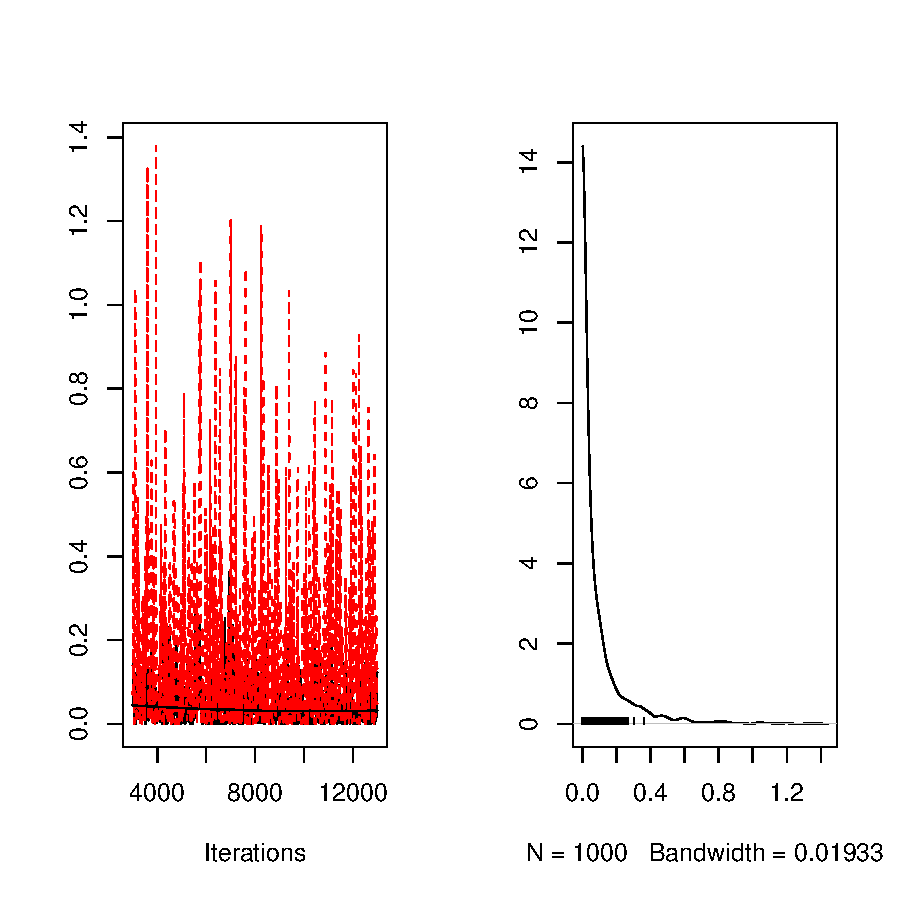
\includegraphics{Lecture8-020}
\end{center}
\caption{Between mother variation in sex ratio with the residual variance fixed at 1 (black trace) and 10 (red trace).}
\label{sexratio2-fig}
\end{figure}

The two models appear to give completely different posteriors (Figure \ref{sexratio2-fig}) but rescaling indicates that they are very similar (Figure \ref{sexratio3-fig}), even though the different residual variances induce different priors on the scaled variances:

\begin{Schunk}
\begin{Sinput}
> c2 <- (16 * sqrt(3)/(15 * pi))^2
> plot(mcmc.list(m7b.1$VCV[, 1]/(1 + c2 * m7b.1$VCV[, "units"]), 
+     m7b.3$VCV[, 1]/(1 + c2 * m7b.3$VCV[, "units"])))
\end{Sinput}
\end{Schunk}

\begin{figure}[!h]
\begin{center}
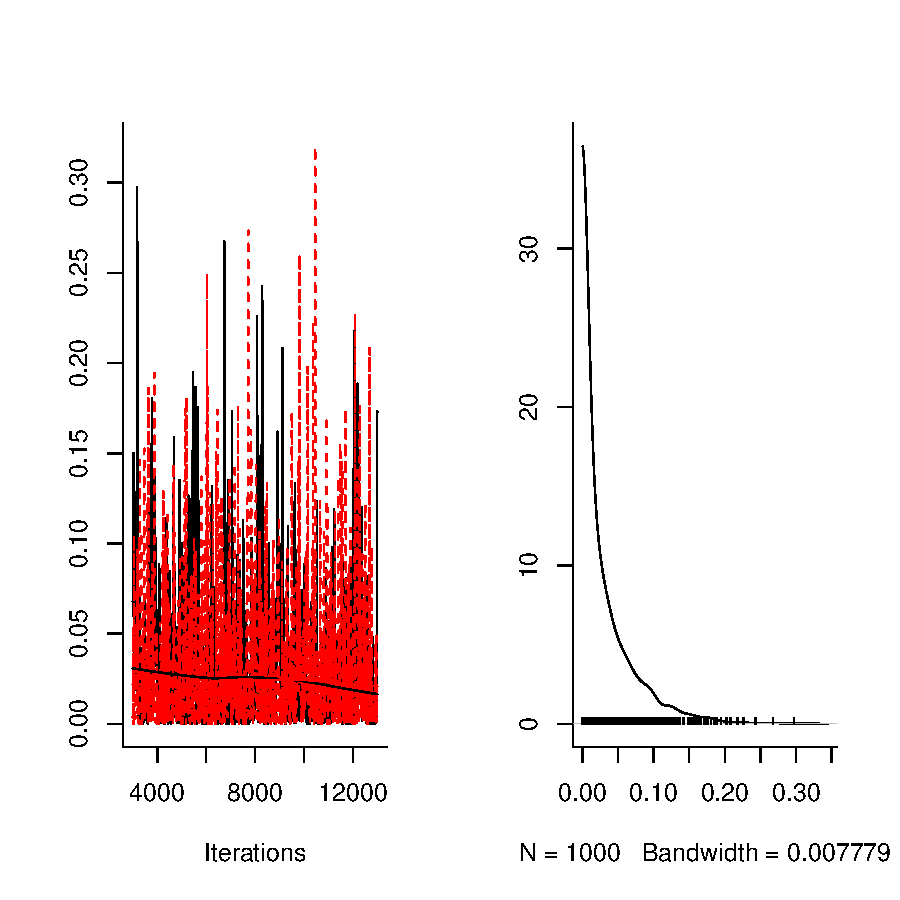
\includegraphics{Lecture8-022}
\end{center}
\caption{Between mother variation in sex ratio with the residual variance fixed at 1 (black trace) and 10 (red trace) but with both estimates rescaled to what would be observed under no residual variance.}
\label{sexratio3-fig}
\end{figure}

Despite their similarity however, the mixing properties of the second chain are much better \citep{vanDyk.2001}:

\begin{Schunk}
\begin{Sinput}
> effectiveSize(m7b.1$VCV[, 1]/(1 + c2 * m7b.1$VCV[, "units"]))
\end{Sinput}
\begin{Soutput}
    var1 
116.9204 
\end{Soutput}
\begin{Sinput}
> effectiveSize(m7b.3$VCV[, 1]/(1 + c2 * m7b.3$VCV[, "units"]))
\end{Sinput}
\begin{Soutput}
    var1 
835.2753 
\end{Soutput}
\end{Schunk}

Although the chain mixes faster as the residual variance is set to be larger, numerical problems are often encountered because the latent variables can take on extreme values. For most models a variance of 1 is safe, but care needs to be taken so that the absolute value of the latent variable is less than 20 in the case of the logit link and less than 7 for the probit link. If the residual variance is not fixed, but has an alternative proper prior placed on it, then the Metropolis-Hastings proposal distribution for the latent variables may not be well suited to the local properties of the conditional distribution, and the acceptance ratio may fluctuate widely around the optimal 0.44. This can be fixed by using the slice sampling methods outlined in \citet{Damien.1999} by passing \texttt{slice=TRUE} to \texttt{MCMCglmm}. Slice sampling can also be more efficient even if the prior is fixed at some value: 
 
\begin{Schunk}
\begin{Sinput}
> m7b.4 <- MCMCglmm(sex ~ 1, random = ~dam, data = BTdata, family = "categorical", 
+     prior = prior3b, verbose = FALSE, slice = TRUE)
> effectiveSize(m7b.4$VCV[, 1]/(1 + c2 * m7b.3$VCV[, "units"]))
\end{Sinput}
\begin{Soutput}
    var1 
798.2359 
\end{Soutput}
\end{Schunk}

\ifalone
\bibliographystyle{JSS}
\bibliography{JarLib}
\end{document}
\else
\fi

